
\section{Capacity limit analysis}

\subsection{zero-dispersion solution}
We can consider a two channel case with zero-dispersion optical fiber.
$$
\begin{array}{r}
\frac{\partial A_{1}}{\partial z} = i \gamma_{1}\left(\left|A_{1}\right|^{2}+2\left|A_{2}\right|^{2}\right) A_{1} \\
\frac{\partial A_{2}}{\partial z}+d \frac{\partial A_{2}}{\partial T} =i \gamma_{2}\left(\left|A_{2}\right|^{2}+2\left|A_{1}\right|^{2}\right) A_{2}
\end{array}
$$
where $T$ is measured in a reference frame moving at the speed.The solution:
$$
A_{1}(L, T)=A_{1}(0, T) e^{i \phi_{1}}, \quad A_{2}(L, T)=A_{2}(0, T-d L) e^{i \phi_{2}}
$$
where 
$$
\begin{array}{l}
\phi_{1}(T)=\gamma_{1}\left(L\left|A_{1}(0, T)\right|^{2}+2 \int_{0}^{L}\left|A_{2}(0, T-z d)\right|^{2} d z\right) \\
\phi_{2}(T)=\gamma_{2}\left(L\left|A_{2}(0, T)\right|^{2}+2 \int_{0}^{L}\left|A_{1}(0, T+z d)\right|^{2} d z\right) .
\end{array}
$$
We can not infer the value of $\phi_1$ using only the information of $A_1$. We need some prior knowlege about $A_2$, for example the power of $A_2$.

\textbf{different scale}: \\
change variable:
$$
\tau = \frac{t}{T_0}, z' = \frac{z}{L}
$$
$$
\frac{\partial u}{\partial z^{\prime}}=-\frac{i s L}{2 L_{D}} \frac{\partial^{2} u}{\partial \tau^{2}}+\frac{i L}{L_{\mathrm{NL}}} e^{-\alpha z}|u|^{2} u
$$
where $T_0$ is the symbol time,$s=sign(\beta_2)$.Two characteristic length for dispersion and nonlinear effect:
$$
L_D = \frac{T_0^2}{|\beta_2|}, \ L_{NL} = \frac{1}{\gamma P_0}
$$

\begin{figure}[ht]
\centering
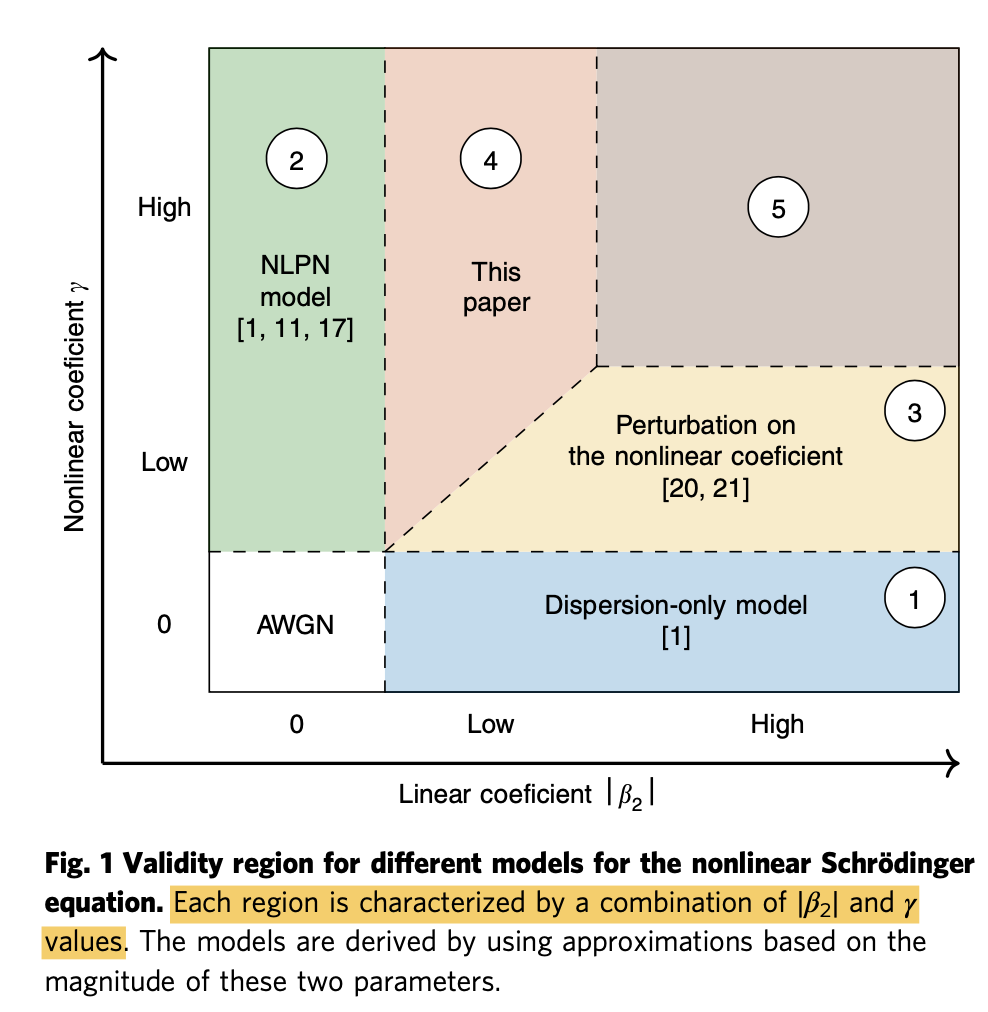
\includegraphics[width=0.6\linewidth]{img/model_class.png}
\caption{model class\cite{2020_weak_dsp_nature}}
\label{model class}
\end{figure}
\begin{itemize}
\item Assumption,model
	\begin{enumerate}
	\item model validity region.(dispersion vs nonlinear term)
	\item noise term.(exist or not)
	\item signal assumption.(Gaussian or others)
	\item method.(RP,LP,Voterra series,simulations..)
	\item Gaussian estimate.(treat the XPM,FWM as gaussian noise.)
	\item single channel or WDM.
	\item bound.
	\end{enumerate}
\item method
\item Bound
\end{itemize}

\begin{itemize}
\item simple model
\item simulation
\end{itemize}

\begin{theorem}[Pinsker formula]
$$
C_{G} \equiv \log _{2} \frac{\operatorname{Det} \operatorname{diag}\left(C_{\alpha \beta}\right)}{\operatorname{Det} C_{\alpha \beta}}, \quad C_{\alpha \beta} \equiv\left\langle u_{\alpha} u_{\beta}^{*}\right\rangle
$$
where $C_{\alpha\beta}$ is the input-output correlation matrix. This is a lower estimate for shannon capacity.
\end{theorem}

 \begin{table}[ht]
		\centering
		\begin{tabular}{|c|c|c|c|c|c|c|}\hline
			Author & validity region & ASE & signal input & method & Pinsker formula & bound. \\
			\hline
			1993 Splett\cite{splett1993} & 3 & no & Gaussian & RP & yes & FLB \\
			\hline
			2002 narimanov\cite{narimanov2002} & 3 & multi-span & Gaussian & RP & yes & FLB \\
			\hline
			1993 Mecozzi\cite{1993Mecozzi} & 2 & distributed & - & moments & - & - \\
			\hline
			2003 turitsyn\cite{2003turitsyn} & 2 & distributed & Gaussian & path integral & No & ILB \\
			\hline
			2006 Ivkovic\cite{2006Ivkovic} &   &  &  & simulation &  &  \\
			\hline

		\end{tabular}
		\caption{summary of bound: FLB(Finite lower bound), IFB(Infinite lower bound)}
		\label{summary}
\end{table}
\textbf{Add a dimension: single channel or WDM.}

\begin{figure}
\centering
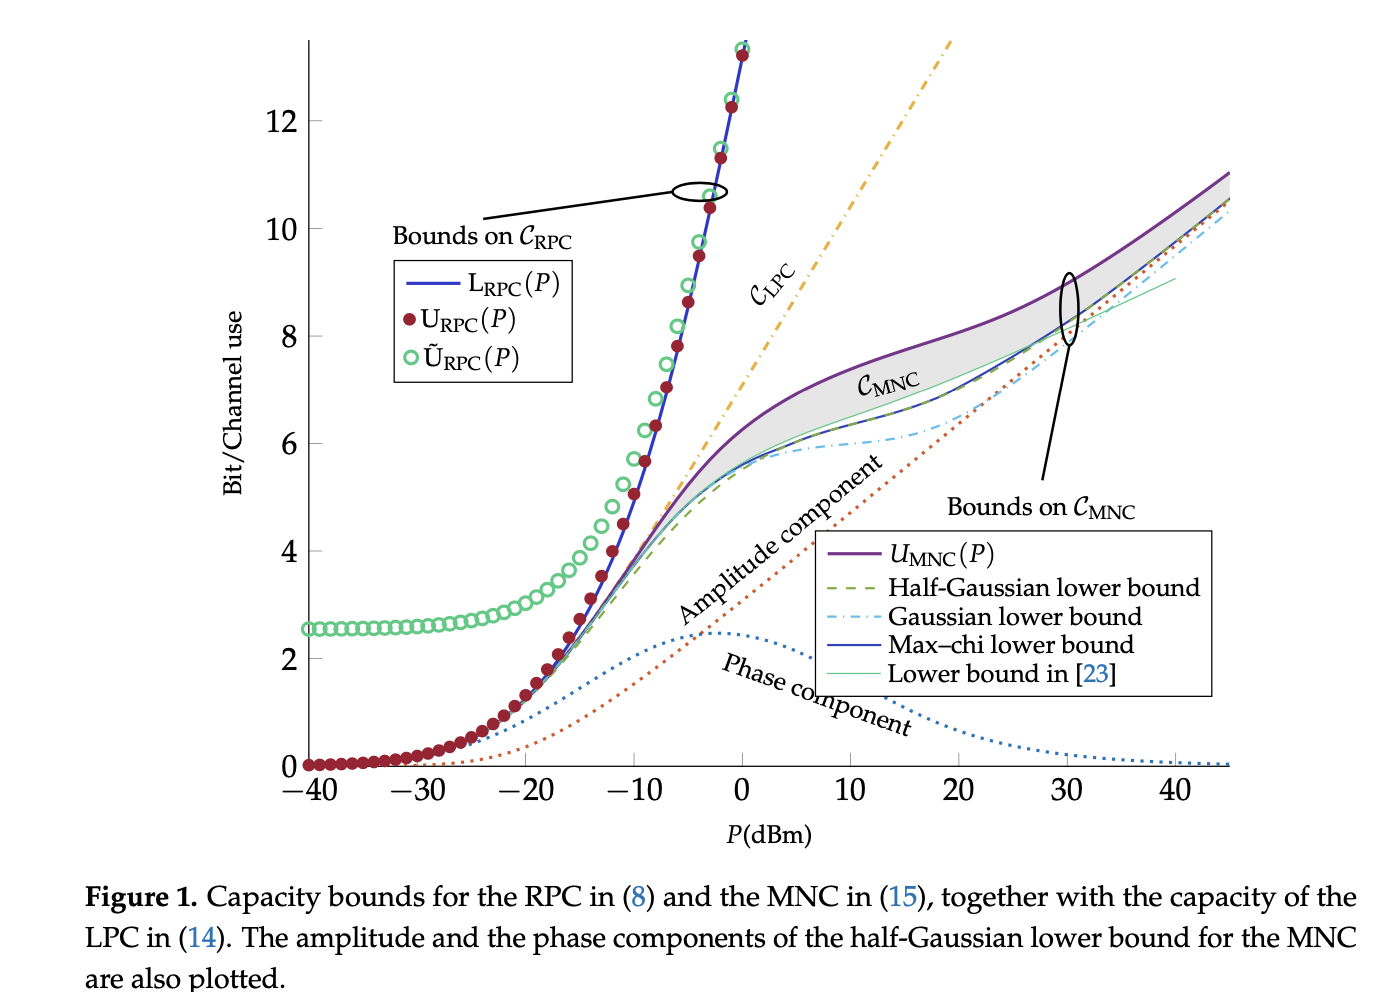
\includegraphics[width=0.8\linewidth]{img/zeros_disp_plot.png}
\caption{zero dispersion case: \textbf{region 2}}
\label{region 2}
\end{figure}

\begin{align*}
n^{\frac{1}{\log n}} = e^{\log n \frac{1}{\log n}} = e^{1} = e
\end{align*}
